%!TEX root=../../autopilot.tex
\section{GUI \& Plots}
\label{sec:ui}

The terminal's GUI controls day-to-day system operation\sidenote{Autopilot uses \href{https://wiki.qt.io/PySide}{PySide}, a wrapper around \href{https://www.qt.io/}{Qt}, to build its GUI.}. It is intended to be a nontechnical frontend that can be used by those without programming experience. 

For each pilot, the terminal creates a control panel that manages subjects, task operation, and plots incoming data. \href{http://docs.auto-pi-lot.com/guide.training.html#creating-a-subject}{Subjects can be managed} through the GUI, including creation, protocol assignment, and metadata editing. Protocols can also be \href{http://docs.auto-pi-lot.com/guide.training.html#creating-a-protocol}{created from within the GUI}. The \hyperref[sec:taskcomponents]{\texttt{PARAMS}} dictionary from a task is used to programmatically generate a series of fields that the user can fill to describe their particular version of the task. The standardized description of tasks not only allows them to be reused between researchers, but also take advantage of the rest of the infrastructure of Autopilot.

The GUI also has a set of basic maintenance and informational routines in its menus, like calibrating water ports or viewing a history of subject weights. The simple callback design and network infrastructure makes adding new GUI functionality straightforward.

\subsection{Plotting}
\label{sec:plotting}

\begin{marginfigure}[-5.5cm]
\begin{minted}[frame=lines,label=Trial Plot,fontsize=\small]{json}
{"data": {
    "target"   : "point",
    "response" : "segment",
    "correct"  : "rollmean"
},
"roll_window" : 50}
\end{minted}
\begin{minted}[frame=lines, label=Continuous Plot,fontsize=\small]{json}
{"data": {
    "target"   : "point",
    "response" : "segment",
    "velocity" : "shaded"
},
"continuous": true}
\end{minted}
\caption{\texttt{PLOT} parameters for Figure \ref{fig:gui}. In both, "target" and "response" data are mapped to "point" and "segment" graphical primitives, but timestamps rather than trial numbers are used for the x-axis in the "continuous" plot (Figure \ref{fig:gui}, bottom). Additional parameters can be specified, eg. the trial plot (Figure \ref{fig:gui}, top) computes rolling accuracy over the past 50 trials}
\label{fig:plotparams}
\end{marginfigure}

Realtime data visualization is critical for monitoring training progress and ensuring that the task is working correctly, but each task has different requirements for visualization. A task that has a subject continuously running on a ball requires a continuous readout of running velocity, whereas a trial-based task only needs to show correct/incorrect responses as they happen. Autopilot solves this problem by assigning the data returned by the task to graphical primitives like points, lines, or shaded areas as specified in a task's \hyperref[sec:taskcomponents]{\texttt{PLOT}} dictionary (taking inspiration from Wilkinson's grammar of graphics\citep{wilkinsonGrammarGraphics2012}).%
%
\begin{figure*}[hb!]
\caption[][-7cm]{Screenshot from a terminal GUI running two different tasks with different plots concurrently. \texttt{pilot\_1} runs 2 subjects: (\texttt{tones} and \texttt{tones\_2}). See Figure \ref{fig:plotparams} for plot description}
\label{fig:gui}
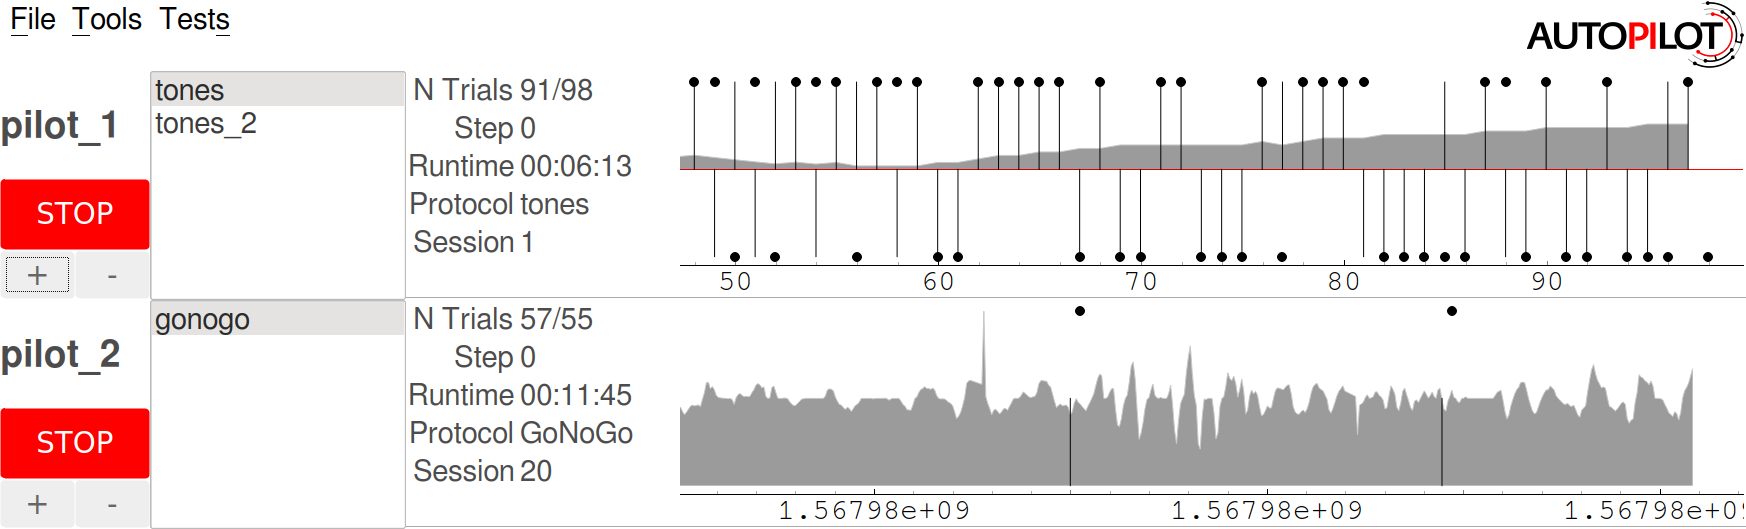
\includegraphics[]{figures/ss_3.png}
\end{figure*}
% keeping in case want to remove param figures
%The top plot displays trial-by-trial information along the x-axis: each dot represents the target response (left = bottom, right = top), and each line segment represents the subject's actual response. A rolling mean of the subject's accuracy is plotted in gray. The bottom plot advances continuously, and displays the subject's velocity (shaded area) as well as the target and actual responses (as in top plot).
\clearpage

